\chapter{Shortest Paths}
Ajur was looking at a map of the cemetery map. He was trying to find a way to go to the water fountain. Then he remembered all the discussions he had been having with Rishnak. Ajur told Jura that there may be a method using Graph Theory to find a path and also the shortest path. Rishnak was watching Ajur looking at the map and realized that discussion of path and shortest path (length of the path from source vertex to the destination vertex) would be an ideal topic to pursue next.

Consider a graph\footnote{In the case of spanning trees, we consider only undirected graphs; however shortest paths, we can consider both undirected and directed graphs.}. Rishnak asked Ajur to find the shortest path from a specified source vertex to a specified destination vertex. Consider the following Graph shown in Figure \ref{12g1}
\begin{figure}
\begin{center}
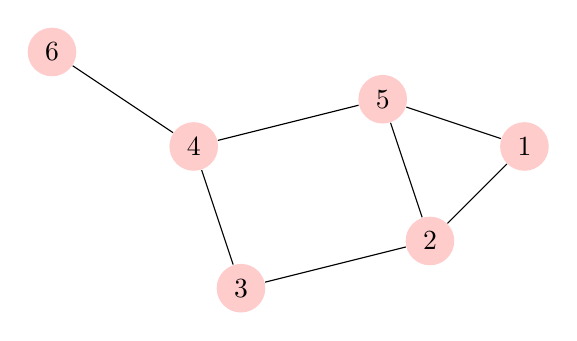
\begin{tikzpicture}
  [scale=.6,auto=left,every node/.style={circle,fill=red!20}]
  \node (n6) at (1,10) {6};
  \node (n4) at (4,8)  {4};
  \node (n5) at (8,9)  {5};
  \node (n1) at (11,8) {1};
  \node (n2) at (9,6)  {2};
  \node (n3) at (5,5)  {3};

  \foreach \from/\to in {n6/n4,n4/n5,n5/n1,n1/n2,n2/n5,n2/n3,n3/n4}
    \draw (\from) -- (\to);

\end{tikzpicture}
\caption{ Example Graph, We want to find the shortest path from vertex 1 to vertex 6}\label{12g1}
\end{center}
\end{figure}

Ajur jumped up and down with excitement and said he could draw the shortest path from source vertex (1) to destination vertex (6). Rishnak asked him to draw the graph. Ajur drew the following graph \ref{12g2}

\begin{figure}
\begin{center}
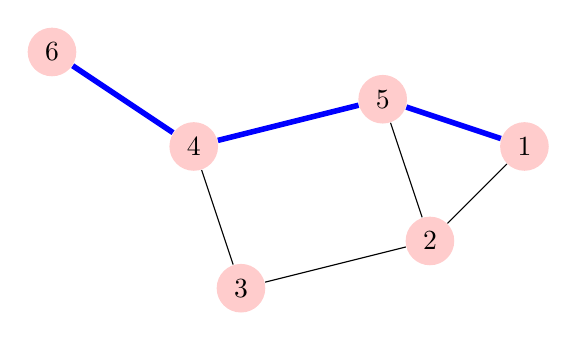
\begin{tikzpicture}
  [scale=.6,auto=left,every node/.style={circle,fill=red!20}]
  \node (n6) at (1,10) {6};
  \node (n4) at (4,8)  {4};
  \node (n5) at (8,9)  {5};
  \node (n1) at (11,8) {1};
  \node (n2) at (9,6)  {2};
  \node (n3) at (5,5)  {3};

  \foreach \from/\to in {n6/n4,n4/n5,n5/n1}
    \draw [line width=2 pt,color=blue] (\from) -- (\to);
\foreach \from/\to in {n3/n4,n3/n2,n2/n1,n2/n5}
    \draw  (\from) -- (\to);

\end{tikzpicture}
\caption{ Example Graph, Shortest Path (of length 3) from vertex 1 to vertex 6 in Graph \ref{12g1} - shortest path is drawn in thick lines.}\label{12g2}
\end{center}
\end{figure}

Rishnak admired Ajur's enthusiasm but wanted to find out whether Ajur can find a general method of finding the shortest path from a source vertex to a destination vertex.

Rishnak suggested the following method similar to that of finding any spanning tree \ref{12a1}

\begin{figure} 
\begin{enumerate}
\item Iniitally label all the vertieces as $\infty$. Label of a vertex,$y$ gives the distance from the source vertex to the vertex $y$.  Label the source vertex as 0. The distance from the source vertex to itself is 0. Start from the source vertex. Include that vertex in a queue. \footnote{ In a queue, you can only put in the rear and take from the front.} 
\item Remove the vertex from the front of the queue. find all vertices $v$, (not yet labeled) that is adjacent to the removed vertex ($w$) in the queue. Label all these vertices as one more than the label of $w$ . Include that edge, $(v,w)$ in the spanning tree.
\item Repeat the above step till all the vertices are in the bag.
\end{enumerate}
\caption{Finding a shortest Path from source vertex to a sink vertex.}\label{12a1}
\end{figure}